%!TEX program = xelatex

\documentclass[11pt,titlepage]{report}
%!TEX root = main.tex

\usepackage[T1]{fontenc}
\usepackage{lmodern}
\usepackage[svgnames]{xcolor}
\usepackage{fontspec} % XeLaTeX required!
\usepackage{graphicx}
\usepackage{tikz}
\usepackage{pifont}
\usepackage[some]{background}
\usepackage{xltxtra} 
\usepackage{setspace}
\usepackage[absolute]{textpos}
\usepackage[latin1]{inputenc}
\usepackage[english]{babel}
\usepackage{graphicx}
\usepackage{wrapfig}
\usepackage{fullpage}
\usepackage[margin=1in]{geometry}
\usepackage{float}
\usepackage{url}
\usepackage{multicol}
\usepackage{hyperref}
\usepackage{titlepic}
\usepackage{standalone}
\usepackage{siunitx}
\usepackage{booktabs}
\usepackage{amsmath}
\usepackage{unicode-math}
\usepackage{verbatim}
\usepackage{enumitem}
\usepackage{listings}
\usepackage{multirow}
\usepackage{pgfplots}
\pgfplotsset{compat=1.8}
\usepackage{caption} 
\usepackage[parfill]{parskip}
\usepackage{import}
\usepackage[backend=bibtexu,texencoding=utf8,bibencoding=utf8,style=ieee,sortlocale=en_GB,language=auto]{biblatex}
\usepackage[strict,autostyle]{csquotes}
\usepackage{pdfpages}
%\usepackage{enumerate}
%\captionsetup[table]{skip=10pt}

\input{../../library/style}
\addbibresource{../../library/bibliography.bib}

% Matrix and vector notation
\newcommand{\mat}[1]{\mathbf{#1}}
\let\vec\vecold
\newcommand{\vec}[1]{\mathbf{\underline{#1}}}
\newcommand{\tr}[1]{#1^{\text T}}

\begin{document}

\chapter{Assignment 1}
\section{Car model}
\begin{figure}[H]
	\centering
	\begin{tikzpicture}[node distance=2cm]
		\bgComponentNoBond{Se}{$S_e:u$}
		\bgComponent{}{1-1}{1}{right of=}{Se}{inbond}
		\bgComponent{}{mass}{$I:m$}{above of=}{1-1}{inbond}
		\bgComponent{}{res}{$R:\rho$}{right of=}{1-1}{inbond}
	\end{tikzpicture}
	\caption{Bond graph representation of the car model}
	\label{fig:ass-1-bond-simple}
\end{figure}

The second-order state-space model fitting the bond graph drawn in Figure~\ref{fig:ass-1-bond-simple} is given by

\begin{align}
	\dot{\vec{x}} = \frac{d}{dt}
	\begin{bmatrix}
		q_m \\
		f_m
	\end{bmatrix} &= \mat{A} \vec{x} + \mat{B} \vec{u} =
	\begin{bmatrix}
		0 & 1 \\
		0 & -\frac{\rho}{m}
	\end{bmatrix}
	\begin{bmatrix}
		q_m \\
		f_m
	\end{bmatrix} +
	\begin{bmatrix}
		0 \\
		\frac{1}{m}
	\end{bmatrix} u \\
	\vec{y} = q_m &= \mat{C} \vec{x} + \mat{D} \vec{u} =
	\begin{bmatrix}
		1 & 0
	\end{bmatrix}
	\begin{bmatrix}
		q_m \\
		f_m
	\end{bmatrix}.
\end{align}

The eigenvalues with corresponding eigenvectors of our state-space model are

\begin{equation}
	\lambda_1 = 0\text{ with }
	\vec{v}_1 = \begin{bmatrix}
		1 \\
		0
	\end{bmatrix},
\end{equation}

\begin{equation}
	\lambda_2 = -\frac{\rho}{m}\text{ with }
	\vec{v}_2 = \begin{bmatrix}
		-\frac{m}{\rho} \\
		1
	\end{bmatrix}.
\end{equation}

Since we have two independent eigenvectors, $\lambda_2 < 0$ and $\lambda_1 = 0$, our system is marginally stable. To investigate the controllability and observability, we used the fact that a pair $(\mat{A},\mat{B})$ is controllable if $\mat{V}$ is a square matrix whose colums consist of different eigenvectors of $\mat{A}$ and every element of the vector $\mat{V}^{-1} \mat{B}$ is non-zero. Since

\begin{equation}
	\left[\vec{v}_1 \vec{v}_2 \right]^{-1} \mat{B} = \begin{bmatrix}
		\frac{1}{m} \\
		\frac{1}{\rho}
	\end{bmatrix}
\end{equation},

we can conclude controllability. Recall that a system is observable, if $(\tr{\mat{A}},\tr{\mat{C}})$ is controllable. Let $\vec{u}_1$ and $\vec{u}_2$ denote the eigenvectors of $\tr{\mat{A}}$, then

\begin{equation}
	\left[\vec{u}_1 \vec{u}_2 \right]^{-1} \tr{\mat{C}} = \begin{bmatrix}
		-\frac{m}{\rho} \\
		\frac{m}{\rho}
	\end{bmatrix}
\end{equation}.

Now we can also conclude observability.




\end{document}